\begin{frame}{x86-64 page table entries (1)}
\begin{tikzpicture}
\node[inner sep=0mm] (tp) {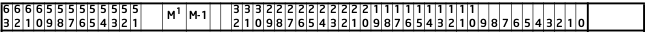
\includegraphics[width=14cm]{../vm/pte-tbl-top}};
\node[below=-.5mm of tp,inner sep=0mm] {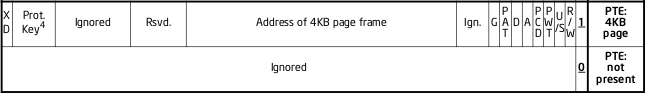
\includegraphics[width=14cm]{../vm/pte-tbl-bottom}};
\end{tikzpicture}
\begin{itemize}
    \small
    \item present = valid\tikzmark{present}
    \item R/W = writes allowed?
    \item U/S = user-mode allowed? (``user/supervisor'')
    \item XD = execute-disable?
    \item A = accessed?\tikzmark{accessed} (MMU sets to 1 on page read/write)
    \item D = dirty?\tikzmark{dirty} (MMU sets to 1 on page write)
\end{itemize}
\begin{tikzpicture}[overlay,remember picture]
    \begin{visibleenv}<all:2>
    \node[my callout=accessed,anchor=south west] at ([xshift=-2cm,yshift=-1cm]pic cs:accessed) {
        helps support replacement policies for swapping
    };
    \end{visibleenv}
    \begin{visibleenv}<all:3>
    \node[my callout=dirty,anchor=south west] at ([xshift=-2cm,yshift=-1cm]pic cs:dirty) {
        helps support writeback policy for swapping
    };
    \end{visibleenv}
\end{tikzpicture}
\end{frame}

\begin{frame}{x86-64 page table entries (2)}
\begin{tikzpicture}
\node[inner sep=0mm] (tp) {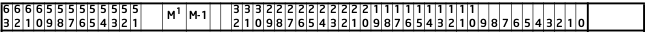
\includegraphics[width=14cm]{../vm/pte-tbl-top}};
\node[below=-.5mm of tp,inner sep=0mm] {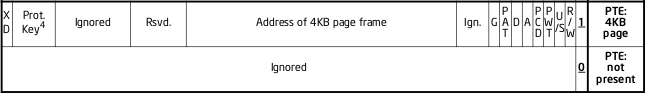
\includegraphics[width=14cm]{../vm/pte-tbl-bottom}};
\end{tikzpicture}
\begin{itemize}
    \small
\item G = global?\tikzmark{global} (shared between all page tables)
\item PWT, PCD, PAT = control how caches work when accessing physical page:
    \begin{itemize}
    \item can disable using the cache entirely
    \item can disable write-back (use write-through instead)
    \item multicore-related cache settings
    \item (and some other settings)
    \end{itemize} 
\end{itemize}
\begin{tikzpicture}[overlay,remember picture]
    \begin{visibleenv}<all:2>
    \node[my callout=global,anchor=south west] at ([xshift=-2cm,yshift=-1cm]pic cs:global) {
        CPU won't evict TLB entries on most page table base registers changes
    };
    \end{visibleenv}
\end{tikzpicture}
\end{frame}
